\graphicspath{{cvxpyth/}}

\chapter{Differentiable \cvxpy Optimization Layers}
\label{sec:cvxpyth}

% TODO: Make sure this is in the intro:
%
% We briefly discuss why this differentiable \cvxpy layer
% adds significant modeling convenience for prototyping
% optimization layers.
% \begin{enumerate}
% \item \cvxpy is a powerful prototyping tool on its own
%   and is widely used in the optimization community because
%   transforming problems to the standard form required by
%   solvers is cumbersome and error-prone.
%   To use the existing optimization layers,
%   users needed to hand-implement a solver for their optimization problem
%   or transform it to a standard to be used with
%   libraries such as \verb!qpth!.
%   Doing this transformation manually is feasible for small
%   optimization problems but becomes a significant
%   development bottleneck for more sophisticated
%   problems and is something that \cvxpy handles automatically.
% \item Implicitly differentiating the KKT conditions
%   or fixed-point equations for optimization problems
%   can be an involved process. For the same reasons
%   why having \cvxpy is useful for the forward pass,
%   our contribution provides a similarly convenient
%   backward pass implementation than users no longer
%   have to implement by hand.
% \end{enumerate}

This thesis has presented differentiable optimization layers
as a powerful class of operations for end-to-end learning
that allow more specialized domain knowledge to be integrated
into the modeling pipeline in a differentiable way.
Convex optimization layers can be represented as
\begin{equation}
  \label{eq:optimization-layer}
  z_{i+1} = \argmin_z f_\theta(z, z_i)\;
  {\rm s.t.}\;z\in \CC_\theta(z_i)
\end{equation}
where $z_i$ is the previous layer,
$f$ is a convex objective function parameterized
by $\theta$, and $\CC$ is a convex constraint set.
From the perspective of end-to-end learning,
convex optimization layers can be seen
as a module that outputs $z_{i+1}$ and has parameters
$\theta$ that can be learned with gradient descent.
We note that the convex case captures many
of the applications above, and can be used as
a building block for differentiable non-convex
optimization problems.

Implementing optimization layers can be non-trivial as explicit
closed-form solutions typically do not exist.
The forward pass needs to call into an optimization
problem solver and the backward pass typically
\emph{cannot} leverage automatic differentiation.
The backwards pass is usually implemented by implicitly
differentiating the KKT conditions of the optimization problem
as done in bilevel optimization
\citep{gould2016differentiating,kunisch2013bilevel},
sensitivity analysis
\citep{bertsekas1999nonlinear,fiacco1990sensitivity,bonnans2013perturbation},
and in our OptNet approach \cref{sec:optnet}.
Thus to implement an optimization layer, users
have to manually implement the backwards pass,
which is cumbersome and error-prone,
or use an existing optimization problem layer such as
the differentiable QP layer from \cref{sec:optnet},
which is not capable of exploiting problem-specific
structures, uses dense operations, and requires
the user to manually transform their problem into
a standard form.

In this chapter, we show how to turn the \cvxpy
modeling language \citep{diamond2016cvxpy} into
a differentiable optimization layer and
implement our method in PyTorch \citep{paszke2017automatic}.
This allows users to express convex optimization layers in
the intuitive \cvxpy modeling language without needing
to manually implement the backward pass.

We make \cvxpy differentiable with respect to the
\texttt{Parameter} objects provided to the optimization problem
by making internal \cvxpy components differentiable.
This involves differentiating the reduction from the \cvxpy
language to the problem data of a cone program in standard form
and then differentiating through the cone program.
We show how to differentiate through cone programs by
implicitly differentiating the residual map from
\citet{busseti2018solution},
which is of standalone interest as
this shows how to differentiate through optimization
problems with non-polyhedral constraints.

\section{Background}
\subsection{The \cvxpy modeling language}
\label{sec:bg:cvxpy}
\cvxpy \citep{diamond2016cvxpy}
is a domain-specific modeling language
based on disciplined convex programming
\citep{grant2006disciplined}
that allows users to express optimization problems
in a more natural way than the standard form
required my most optimization problem solvers.
\cvxpy works by transforming the optimization
problem from their domain-specific language to a
standard (or canonical) form that is passed into
a solver. This inner canonicalized problem is
then solved and the results are returned to
the user. In this chapter, we focus on the
canonicalization to a cone program, which is
one of the most commonly used modes as most convex
optimization problems can be expressed as a cone program,
although we note that our method can be
applied to other \cvxpy solvers.
\cref{fig:overview} overviews the relevant
\cvxpy components.

\subsection{Cone Preliminaries}
A set $\mathcal{K}$ is a \emph{cone}
if for all $x\in\mathcal{K}$ and $t>0$,
$tx\in\mathcal{K}$.
The \emph{dual cone} of a cone $\mathcal{K}$ is
$$\mathcal{K}^* =\menge{y}{\inf_{x\in \mathcal{K}} y^\top x\ge 0}.$$
Commonly used cones include the
nonnegative orthant $\menge{x}{x\geq 0}$,
second-order cone $\menge{(x,t)\in\RR^n_+}{t\geq ||x||_2}$,
positive semidefinite cone $\{X=X^\top \succeq 0\}$,
and
exponential cone
\begin{equation}
  \menge{(x,y,z)}{y>0, ye^{x/y} \leq z} \cup
  \menge{(x,0,z)}{x\leq 0, z\geq 0}
\end{equation}
We can also create a cone from the Cartesian
products of simpler cones as
$\mathcal{K}=\mathcal{K}_1\times \ldots \times\mathcal{K}_p$.

\subsection{Cone Programming}
Most convex optimization problems can be represented and
efficiently solved as a cone program that uses
the nonnegative orthant, second-order cone,
positive semidefinite cone, and exponential cones.
This applicability makes them a commonly used internal
solver for \cvxpy, which implements many of the
well-known transformations from problems to their
conic form.
In the following we state properties of cone programs
and useful definitions for this chapter.
More details about cone programming can be found in
\citet{boyd2004convex,ben2001lectures,busseti2018solution,odonoghue2016conic,lobo1998applications,alizadeh2003second}.

In their primal (P) and dual (D) forms,
cone programs can be represented as \\
\begin{minipage}{0.45\textwidth}
  \begin{equation*}
    % \tag{P}
    \begin{array}{lll}
      \text{(P)}\;\; \xstar, \sstar =
      &\argmin_{x,s} &c^\top x\\
      &\subjectto &  Ax+s=b\\
      &  &s\in  \mathcal{K}
    \end{array}
  \end{equation*}
  \vspace{3mm}
\end{minipage}
\hfill
\begin{minipage}{0.5\textwidth}
  \begin{equation}
    \label{eq:cp}
    % \tag{D}
    \begin{array}{lll}
      \text{(D)}\;\; \ystar =
      & \argmax_y & b^\top y\\
      &\subjectto & A^\top y+c=0\\
      &&y\in  \mathcal{K}^*
    \end{array}
  \end{equation}
  \vspace{3mm}
\end{minipage}
where $x\in\R^n$ is the \emph{primal variable},
$s\in\R^m$ is the \emph{primal slack variable},
$y\in\R^m$ is the \emph{dual variable}.
and $\mathcal{K}$ is a nonempty, closed, convex cone
with dual cone $\mathcal{K}^*$.

\textbf{The KKT optimality conditions.}
The Karush--Kuhn--Tucker (KKT) conditions for the
cone program in \cref{eq:cp} provide
necessary and sufficient conditions for optimality
and are defined by
\begin{equation}
\label{eq:cp-kkt}
Ax +s =b, \quad
A^\top y + c = 0, \quad
s \in \mathcal{K}, \quad
y \in \mathcal{K}^*, \quad
s^\top y = 0.
\end{equation}
The complimentary slackness condition $s^\top y = 0$ can
alternatively be captured with a condition that
makes the duality gap zero $c^\top x + b^\top y = 0$.

\textbf{The homogenous self-dual embedding.}
\citet{ye1994nl} converts the primal and cone dual programs
in \cref{eq:cp} into a single feasibility problem called
the homogenous self-dual embedding, which is defined by
\begin{equation}
\label{e:hsde:1}
Qu = v, \quad u \in \mathbfcal{K},
\quad v \in \mathbfcal{K}^*, \quad u_{m+n+1} +
 v_{m+n+1} >0,
\end{equation}
where
\[
\mathbfcal{K} = \RR^n \times \mathcal{K}^*\times \RR_+, \quad
\mathbfcal{K}^* = \{0\}^n\times \mathcal{K}\times \RR_+,
\]
and $Q$ is the skew-symmetric matrix
\[
	Q = \begin{bmatrix}
		0 & A{^\top} & c\\
		-A & 0 & b \\
		-c{^\top} & -b{^\top} & 0
	\end{bmatrix}.
\]
A solution to this embedding problem $(\ustar, \vstar)$
can be used to determine the solution of a conic
problem, or to certify the infeasibilty of the
problem if a solution doesn't exist.
If a solution exists, then
$\ustar=(\xstar/\tau,\ystar/\tau,\tau)$
and
$\vstar=(0, \sstar/\tau, 0)$.

\textbf{The conic complementarity set.}
The \emph{conic complementarity set} is defined by
\begin{equation}
\label{eq:con:com:set}
\mathcal{C} = \menge{(u,v) \in
  \mathbfcal{K} \times \mathbfcal{K}^* }{u^\top v = 0}.
\end{equation}
We denote
the Euclidean projection onto
$\mathbfcal{K}$ with $\Pi$
and
the Euclidean projection onto
$-\mathbfcal{K}^*$ with $\Pi^*$.
\citet{moreau1961decomposition} shows that
$\Pi^*=I-\Pi$.

\textbf{Minty's parameterization of the complementarity set.}
Minty's parameterization of $\mathcal{C}$
$M: \RR^{m+n+1} \to \mathcal{C}$ as
$M(z) = (\Pi z, -\Pi^* z)$.
This parameterization is invertible with
$M^{-1}(u,v) = u-v$.
See
\citet[Corollary~31.5.1]{rockafellar1970convex}
and \citet[Remark~23.23(i)]{bauschke2017convex}
for more details.
The homogeneous self-dual embedding can be expressed
using Minty's parameterization as
$-\Pi^* z=Q\Pi z$ where $z_{m+n+1} \neq 0$.

\textbf{The residual map of Minty's parameterization.}
\label{sec-residual-map}
\citet{busseti2018solution} defines the
\emph{residual map} of Minty's parameterization
$\Res: \RR^{m+n+1}\to \RR^{m+n+1}$
as
\begin{equation}
\label{eq-residual}
\Res(z) = Q\Pi z+\Pi^*z=((Q-I)\Pi+I)z.
\end{equation}
and shows how to compute the derivative of it
when $\Pi$ is differentiable at $z$ as
\begin{equation}
\label{eq:res:der}
\DD_z\Res(z) =(Q-I)\DD_z\Pi(z) +I,
\end{equation}
where $z\in \RR^{m+n+1}$.
The cone projection differentiation $\DD_z \Pi(z)$
can be computed as described in
\citet{ali2017semismooth}.

\textbf{The Splitting Conic Solver (SCS).}
SCS \citep{odonoghue2016conic} is an efficient way of solving
general cone programs by using the alternating
direction method of multipliers (ADMM)
\citep{boyd2011distributed} and is a commonly used
solver with \cvxpy.
In the simplified form, each iteration
of SCS consists of the following three steps:
\begin{equation}
\begin{array}{rcl}
\tilde u^{k+1} &=& (I + Q)^{-1} (u^k + v^k )\\[1ex]
u^{k+1} &=& \Pi\left(\tilde u^{k+1} - v^k\right) \\[1ex]
v^{k+1} &=&  v^k - \tilde u^{k+1} + u^{k+1}.
\end{array}
\label{eq:scs}
\end{equation}

The first step projects onto an affine subspace,
the second projects onto the cone
and the last updates the dual variable.
In this paper we will mostly focus on solving the
affine subspace projection step. \citet[Section 4.1]{odonoghue2016conic}
shows that the affine subspace projection can be
reduced to solving linear systems of the form
\begin{equation}
\label{eq:scs-linsys}
\begin{bmatrix}
I & -A^\top \\
-A & -I  \\
\end{bmatrix}
\begin{bmatrix} z_x \\ -z_y \end{bmatrix}
=
\begin{bmatrix} w_x \\ w_y \end{bmatrix},
\end{equation}
which can be re-written as
\begin{equation}
  \label{eq:scs-linsys-elim}
  z_x = (I + A^\top A)^{-1}(w_x - A^\top w_y), \quad
  z_y = w_y + A z_x.
\end{equation}

\section{Differentiating \cvxpy and Cone Programs}
\label{sec:cvxpyth:diff-cp}

\begin{figure}[t]
  \centering
  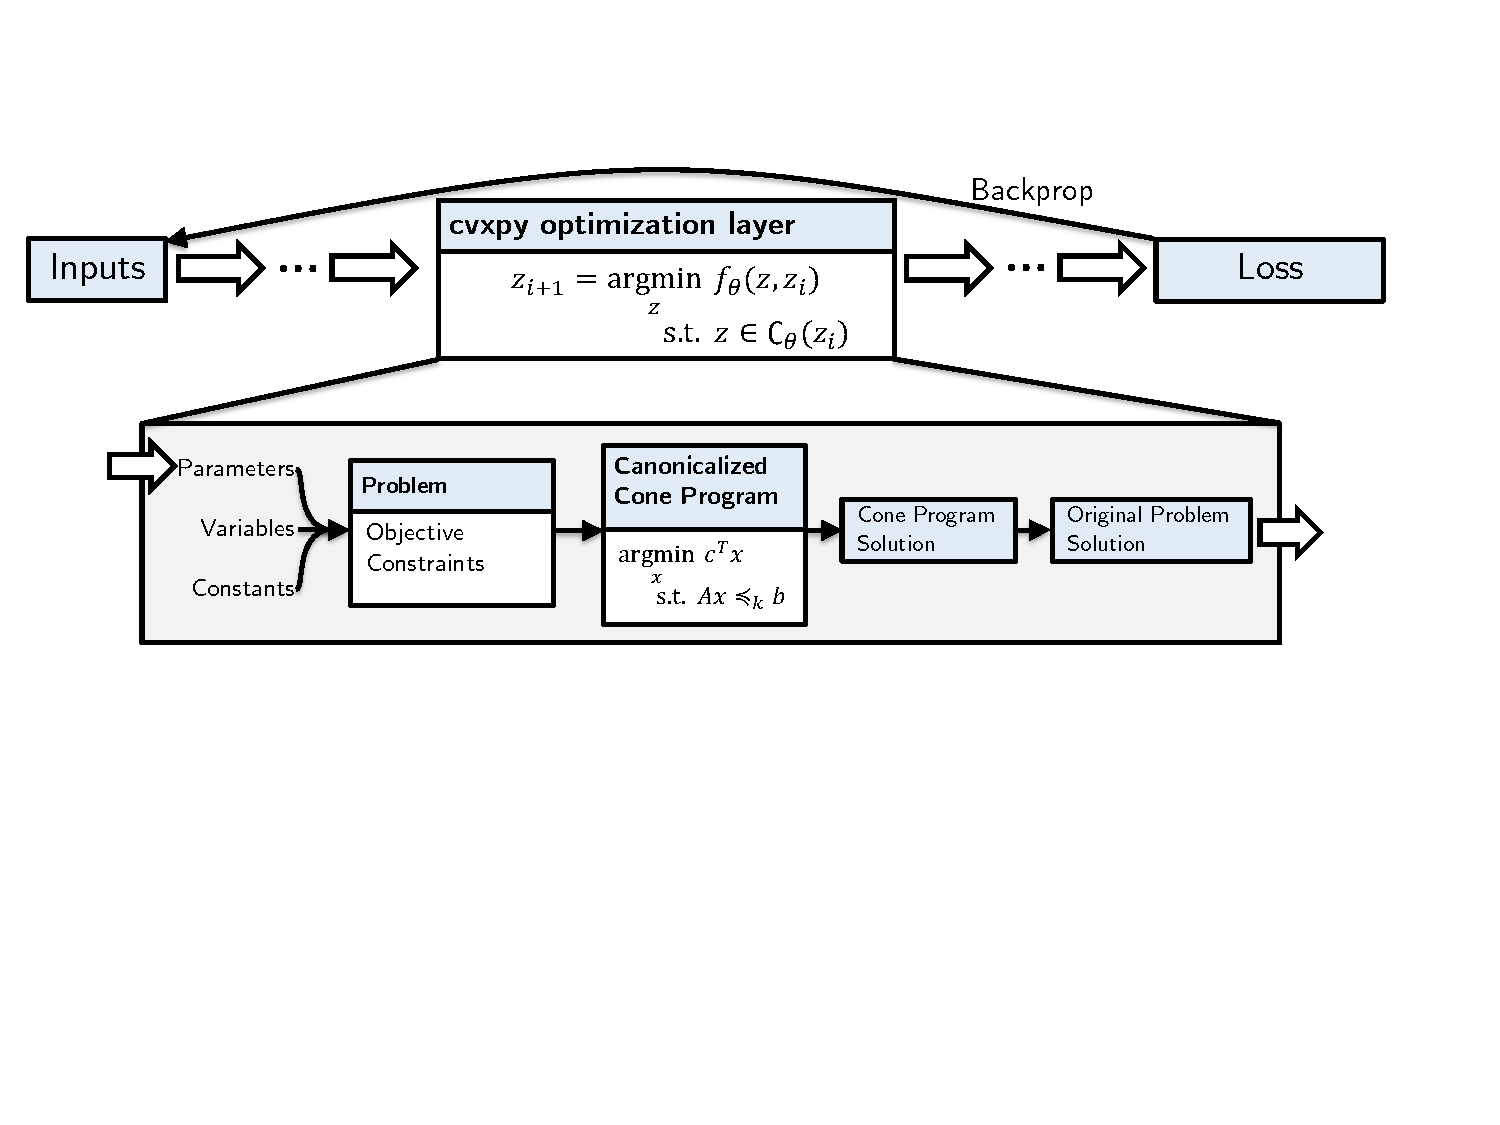
\includegraphics[width=0.9\textwidth]{overview.pdf}
  \caption{
    Summary of our differentiable \cvxpy layer that allows
    users to easily turn most convex optimization problems into
    layers for end-to-end machine learning.
  }
  \label{fig:overview}
\end{figure}

We have created a differentiable \cvxpy layer
by making the relevant components differentiable,
which we visually show in \cref{fig:overview}.
We advocate for making the transformation from the
problem data in the original form to the problem data of
the canonicalized cone problem differentiable
by replacing the numpy operations for this component
with an autodiff framework such as PyTorch \citep{paszke2017automatic}
or TensorFlow \citep{abadi2016tensorflow}.
We then pass this data into a differentiable cone program
solver, which we show how to create in \cref{sec:diff-cp}
by implicitly differentiating the residual map of
Minty's parameterization for the backward pass.
The solution of this cone program can then be mapped
back up to the original problem space in a differentiable
way and returned.

\subsection{Differentiating Cone Programs}
\label{sec:diff-cp}
We consider the argmin of the primal cone program
in \cref{eq:cp} as a function that maps from the
problem data $\theta = \{c, A, b\}$ to the solution $\xstar$.
The approach from \cref{sec:optnet}
that differentiates through convex quadratic programs by
implicitly differentiating the KKT conditions
is difficult to use for cone programs.
This is because the cone constraints in the KKT conditions
in \cref{eq:cp-kkt} make it difficult to form a
set of implicit functions.
Instead of implicitly differentiating the KKT conditions,
we show how to similarly apply implicit
differentiation to the residual map of
Minty's parameterization shown in \citet{busseti2018solution}
to compute the derivative
$\partial \xstar/\partial \theta$.
Furthermore for backpropagation, the full Jacobian is
expensive and unnecessary to form and we show how to
efficiently compute $\partial \ell/\partial \theta$
given $\partial \ell/\partial \xstar$.

\subsubsection{Implicit differentiation of the residual map}
We assume that we have solved the forward pass of the
cone program in \cref{eq:cp} and have a solution
$\xstar, \sstar, \ystar$.
We now show how to compute
$\partial \xstar/\partial \theta$.
This derivation was concurrently considered and done by
\citet{agrawal2019differentiating}.

We construct $\ustar=(\xstar, \ystar, 1)$,
and $\vstar=(0,\sstar, 0)$, and $\zstar=\ustar-\vstar$.
The residual map of Minty's parameterization is zero,
$R(\zstar)=0$, and forms a set of
implicit equations that describe the solution mapping.
Implicit differentiation can be done as described in
\citet{dontchev2009implicit} with
\begin{equation}
  \label{eq:residual-implicit-diff}
  \DD_\theta \zstar =
    -\left(\DD_z \Res(\zstar)\right)^{-1}
    \DD_\theta \Res(\zstar).
\end{equation}
$\left(\DD_z \Res(\zstar)\right)^{-1}$ can be computed
as described in \citep{busseti2018solution}
and $\DD_\theta \Res(\zstar)$ can be analytically computed.
We consider the scaling factor $\tau=z_{m+n+1}=1$ to be
a constant because a solution to the cone program exists.
Finally, applying the chain rule to $\ustar=\Pi \zstar$
gives
\begin{equation}
  \DD_\theta \ustar = (\DD_z \Pi z) \DD_\theta \zstar.
\end{equation}
We note that implicitly differentiating the residual
map captures implicit differentiation of the KKT conditions
as a special case for simple cones such as the zero cone
and non-negative orthant.

The linear system in \cref{eq:residual-implicit-diff}
can be expensive to solve.
In special cases such as quadratic programs
that we discussed in \cref{sec:optnet}
and LQR \cref{sec:empc}, this system can be interpreted
as the solution to another convex optimization problem
and efficiently solved with a method similar to the
forward pass.
This connection is made by interpreting the linear system
solve as a KKT system solve that represents another
optimization problem.
However for general cone programs it is more difficult
to interpret this linear system as a KKT system
because of the cone projections and therefore it
is more difficult to interpret this linear system
solve as an optimization problem.
Following the method of \citet{busseti2018solution},
we advocate for solving the linear system for general
cone programs with LSQR \citep{paige1982lsqr}.

\textbf{Efficiently backpropagating through cone programs.}
When using cone programs as layers in end-to-end learning systems
with some scalar-valued loss function $\ell$,
the full Jacobian $\DD_\theta \xstar$ is expensive
and unnecessary to form and requires solving
$|\theta|$ linear systems.
The Jacobian is only used when applying the chain rule
to obtain $\DD_\theta \ell = (\DD_\xstar\ell) \DD_\theta \xstar$.
We can directly compute $\DD_\theta \ell$ without computing
the intermediate Jacobian by solving a single linear system.
Following the method of \cref{sec:optnet}, we set up the system
\begin{equation}
  \DD_z \Res(\zstar)
\begin{bmatrix}
  d_{z_1} \\
  d_{z_2} \\
  0 \\
\end{bmatrix} = \\
-
\begin{bmatrix}
  \nabla_\xstar \ell \\
  0 \\
  0 \\
\end{bmatrix}.
\end{equation}
Applying the chain rule to $\ustar=\Pi \zstar$ gives
$d_x = d_{z_1}$ and
$d_y = (\DD_z \Pi z) d_{z_2}$.
We then compute the relevant backpropagation derivatives as
\begin{equation}
  \nabla_c \ell = d_x
  \hspace{20mm}
  \nabla_A \ell = d_y \otimes \xstar + \ystar \otimes d_x
  \hspace{20mm}
  \nabla_b \ell = -d_y
\end{equation}

\section{Forward Pass: Efficiently solving batches of
  cone programs with SCS and PyTorch}
\label{sec:cp:efficient}

Na\"ively implemented optimization layers can become
computational bottlenecks when used in a machine learning
pipeline that requires efficiently processing
minibatches of data.
This is because most other parts of the modeling pipeline
involve operations such as linear maps, convolutions,
and activation functions that can quickly be executed
on the GPU to exploit data parallelism across the minibatch.
Most off-the-shelf optimization problem solvers are designed for
the setting of solving a single problem at a time and are not easily
able to be plugged into the batched setting required
when using optimization layers.

To overcome the computational challenges of solving batches
of cone programs concurrently, we have created a batched
PyTorch and potentially GPU-backed backend for the
Splitting Conic Solver (SCS) \citep{odonoghue2016conic}.
The bottleneck of the SCS iterates in \cref{eq:scs}
is typically in the subspace projection part that solves
linear systems of the form
\begin{equation}
  \tilde u^{k+1} = (I + Q)^{-1} (u^k + v^k )
\end{equation}
We have added a new linear system solver backend to the
official SCS C implementation that calls back
up into Python to solve this linear system.

Our cone program layer implementation offers the following
modes for solving a batch of $N$ cone programs
represented in standard form as in \cref{eq:cp} with
as $\theta_i=\{A_i, b_i, c_i\}$
for $i\in\{1, \ldots, N\}$ with SCS.
As common in practice, we assume that the cone programs
have the structure and use the same cones but have
different problem data $\theta_i$.
We empirically compare these modes in \cref{sec:eval}.

\paragraph{Vanilla SCS, serialized.}
This is a baseline mode that is the easiest to implement and sequentially
iterates through the problems $\theta_i$.
This lets us use the vanilla SCS sparse direct and indirect
linear system solvers on the CPU and CUDA, but does
not take advantage of data parallelism.

\paragraph{Vanilla SCS, batched.}
This is another baseline mode that comes from observing that a
batch of cone programs can be represented as
a single cone program in standard form as in \cref{eq:cp} with
variables $x=[x_1^\top, \ldots, x_N^\top]^\top$
and data $A=\mathrm{diag}(A_1, \ldots, A_N)$,
$b=[b_1^\top, \ldots, b_N^\top]^\top$,
and $c=[c_1^\top, \ldots, c_N^\top]^\top$.
This exploits the knowledge that all of the cone programs
can be solved concurrently. The bottleneck of this
mode is still typically in the linear system solve
portion of SCS, which happens using sparse operations
on the CPU or GPU.

\paragraph{SCS+PyTorch, batched.}
In this mode we represent the batch of cone programs as a single
batched cone program use SCS will callbacks up into Python so
that we can use PyTorch to efficiently solve the linear system.
This allows us to keep the $A$ data in PyTorch and potentially
on the GPU without converting/transferring it and passing it
into the SCS.
Specifically we use dense operations and have implemented
direct and indirect methods to solve \cref{eq:scs-linsys-elim}
in PyTorch and then pass the result back down into SCS for the
rest of the operations.
Our direct method uses PyTorch's batched LU factorizations and
solves and our indirect method uses a batched conjugate
gradient (CG) implementation.
These custom linear system solvers are able to explicitly take
advantage of the independence present in the linear systems
that the sparse linear system solvers may not recognize automatically,
and the dense solvers are also useful for dense cone programs,
which come up in the context of differentiable optimization
layers when large portions of the constraints are being learned.

\section{Examples}
\subsection{The ReLU, sigmoid, and softmax}
This section revisits the optimization views of the ReLU,
sigmoid, and softmax from \cref{sec:bg:existing} and shows how
they can be implemented with our cvxpy layer.

\textbf{The ReLU.}
\begin{lstlisting}
_x = cp.Parameter(n)
_y = cp.Variable(n)
obj = cp.Minimize(cp.sum_squares(_y-_x))
cons = [_y >= 0]
prob = cp.Problem(obj, cons)
layer = CvxpyLayer(prob, params=[_x], out_vars=[_y])
\end{lstlisting}

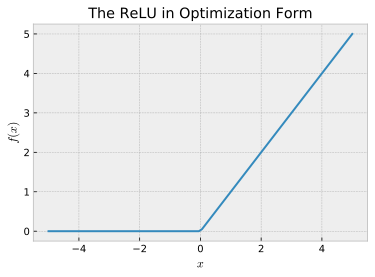
\includegraphics[height=2in]{fs/output_2.pdf}
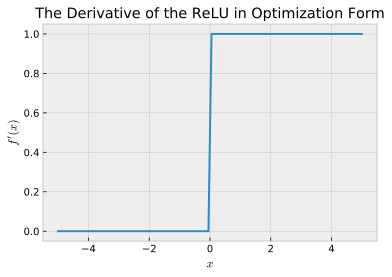
\includegraphics[height=2in]{fs/output_3.pdf}

\textbf{The sigmoid.}
\begin{lstlisting}
_x = cp.Parameter(n)
_y = cp.Variable(n)
obj = cp.Minimize(-_x.T*_y - cp.sum(cp.entr(_y) + cp.entr(1.-_y)))
prob = cp.Problem(obj)
layer = CvxpyLayer(prob, params=[_x], out_vars=[_y])
\end{lstlisting}

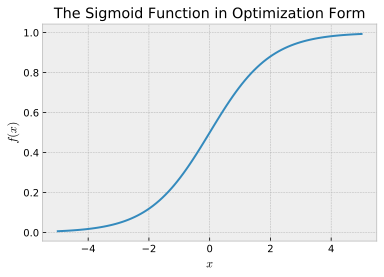
\includegraphics[height=2in]{fs/output_6.pdf}
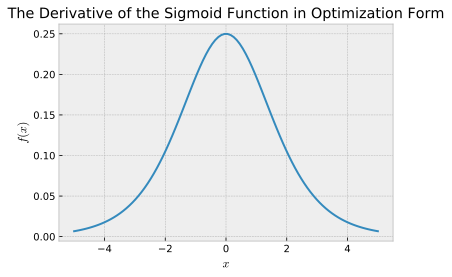
\includegraphics[height=2in]{fs/output_7.pdf}

\newpage
\textbf{The softmax.}
\begin{lstlisting}
_x = cp.Parameter(d)
_y = cp.Variable(d)
obj = cp.Minimize(-_x.T*_y - cp.sum(cp.entr(_y)))
cons = [sum(_y) == 1.]
prob = cp.Problem(obj, cons)
layer = CvxpyLayer(prob, params=[_x], out_vars=[_y])
\end{lstlisting}

\label{sec:cvxpyth:examples}
\subsection{The OptNet QP}

We can re-implement the OptNet QP layer from \cref{sec:optnet}
with our differentiable \cvxpy{} layer in a few lines of code.
The OptNet layer is represented as a convex quadratic program
of the form
\begin{equation}
\begin{split}
x^\star = \argmin_{x} \;\; & \frac{1} {2}x^\top Qx + p^\top x \\
\subjectto \;\; & Ax = b \\
& Gx \leq h \\
\end{split}
\label{eq:cvxpy-qp}
\end{equation}
where $x \in \mathbb{R}^n$ is our optimization variable
$Q \in \mathbb {R}^{n \times n} \succeq 0$
(a positive semidefinite matrix),
$p \in \mathbb {R}^n$,
$A\in \mathbb{R}^{m \times n}$,
$b \in \mathbb{R}^m$,
$G \in \mathbb{R}^ {p \times n}$ and
$h \in \mathbb{R}^{p}$ are problem data.
The \cvxpy{} implementation of this optimization problem is

\begin{lstlisting}
import cvxpy as cp

Q = cp.Parameter((n, n), PSD=True)
p = cp.Parameter(n)
A = cp.Parameter((m, n))
b = cp.Parameter(m)
G = cp.Parameter((p, n))
h = cp.Parameter(p)
x = cp.Variable(n)
obj = cp.Minimize(0.5*cp.quad_form(x, Q) + p.T * x)
cons = [A*x == b, G*x <= h]
prob = cp.Problem(obj, cons)
\end{lstlisting}

Our library allows the \cvxpy{} problem to be turned into
a layer with a single line of code.
\begin{lstlisting}
import cvxpyth

params = [Q, p, A, b, G, h]
out = [x]
layer = cvxpyth.CvxpyLayer(prob, params, out)
\end{lstlisting}

This layer can then be used by passing in the
relevant parameter values:
\begin{lstlisting}
import torch

Lval = torch.randn(nx, nx, requires_grad=True)
Qval = Lval.t().mm(Lval)
pval = torch.randn(nx, requires_grad=True)
Aval = torch.randn(ncon_eq, nx, requires_grad=True)
bval = torch.randn(ncon_eq, requires_grad=True)
Gval = torch.randn(ncon_ineq, nx, requires_grad=True)
hval = torch.randn(ncon_ineq, requires_grad=True)
y = layer(Qval, pval, Aval, bval, Gval, hval)
\end{lstlisting}

\subsection{Ellipsoidally Constrained Problem}
We demonstrate how gradient-based learning can be done with
a \cvxpy layer in this synthetic example.
Consider the ellipsoidally constrained
projection problem
\begin{align*}
\hat y = \argmin_y\;\; &\frac{1}{2}||p-y||_2^2  \\
 {\rm s.t.}\;\; & \frac{1}{2}(y-z)^\top A(y-z) \leq 1
\end{align*}
Suppose we don't know the ellipsoid parameters $\theta=\{A,z\}$
and want to learn them from data.
Then using the MSE for $\ell$, we can randomly initialize
ellipsoids $\theta$ and learn them with gradient steps $\nabla_\theta \ell$.
This is an interesting optimization problem to consider because
it is an example of doing learning with a non-polyhedral cone
program (a SOCP), which prior approaches such as OptNet
could not easily handle.

We implement this layer with:
\begin{lstlisting}
import cvxpy as cp
import cvxpyth as cpth

A = cp.Parameter((n, n), PSD=True)
z = cp.Parameter(n)
p = cp.Parameter(n)
x = cp.Variable(n)
obj = cp.Minimize(0.5*cp.sum_squares(x-p))
cons = [0.5*cp.quad_form(x-z, A) <= 1]
prob = cp.Problem(obj, cons)
params = [p, A, z]
out = [x]
layer = cpth.CvxpyLayer(prob, params, out)
\end{lstlisting}

\begin{figure}[t]
  \centering
  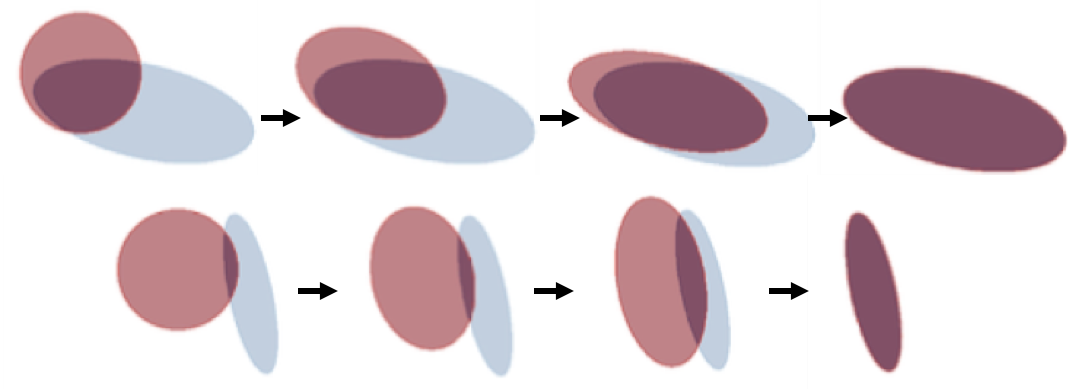
\includegraphics[width=0.6\textwidth]{ellipsoid-frames.png}
  \caption{
    Qualitative results of learning ellipsoidally constrained
    optimization layers.
  }
  \label{fig:ellipsoid-results}
\end{figure}

\cref{fig:ellipsoid-results} shows our empirical results of
learning ellipsoids and visualizes the learning process for
four examples.
Each problem has a true known ellipsoid that we show in blue
and the model's approximation is in red.
Learning starts on the left with randomly initialized
ellipsoids that are updated with gradient steps,
which are shown in the images progressing to the right.

\section{Evaluation}
\label{sec:eval}

In this section we analyze the runtime of our layer's forward
and backward passes compared to hand-written implementations
for commonly used optimization layers.
We will focus on three tasks:

\paragraph{Task 1: Dense QP.}
We consider a QP layer of the form
\cref{eq:cvxpy-qp} with a dense quadratic objective
and dense inequality constraints.
Our default experiment uses a QP with 100 latent
variables, 100 inequality constraints, and
a minibatch size of 128 examples.
We chose this task to understand how the performance
of our \cvxpy{} layer compares to the \qpth implementation
from \citet{amos2017optnet}, which we use as a baseline.
The problem size we consider here is comparable
to the QP problem sizes considered in \citet{amos2017optnet}.
The backwards pass of \qpth is optimized to use a single
batched, pre-factorized linear system solve.

\paragraph{Task 2: Box QP.}
We consider a QP layer of the form
\cref{eq:cvxpy-qp} with a dense quadratic objective
constrained to the box $[-1, 1]^n$.
Our default experiment uses a QP with 100 latent
variables and a minibatch size of 128 examples.
We chose this task to study the impacts of
sparsity on the runtime.
We again use \qpth as the baseline for these experiments.

\paragraph{Task 3: Linear Quadratic Regulator (LQR).}
We consider a continuous-state-action, discrete-time, finite-horizon
LQR problem of the form
\begin{equation}
  \label{eq:cvxpyth:lqr}
  \tau^{\star}_{1:T} = \argmin_{\tau_{1:T}}\;\;
  \sum_{t} \frac{1}{2} \tau_t^\top  C_t \tau_t + c_t^\top  \tau_t \;\;
  \subjectto\;\;
  x_1 = \xinit,\
  x_{t+1} = F_t\tau_t + f_t.
\end{equation}
where $\tau_{1:T} = \{x_t, u_t\}_{1:T}$ is the nominal trajectory,
$T$ is the horizon,
$x_t, u_t$ are the state and control at time $t$,
$\{C_t, c_t\}$ parameterize a convex quadratic cost,
and $\{F_t, f_t\}$ parameterize an affine system
transition dynamics.
We consider a control problem with 10 states,
2 actions, and a horizon of 5.
As a baseline we compare to the differentiable model
predictive control (MPC) solver from
\citep{amos2018differentiable}, which uses batched
PyTorch operations to solve a batch of LQR problems with
the Riccati equations, and then implements the backward
pass with another, simpler, LQR solve with
the Riccati equations.

For each of these tasks we have measured the forward
and backward pass execution times for our layer in
comparison to the baseline implementations.
We have run these experiments on an unloaded system with
an NVIDIA GeForce GTX 1080 Ti GPU and
a four-core 2.60GHz Intel Xeon E5-2623 CPUs hyper-threaded
to eight cores.
We set the number of OpenMP threads to 8 for our experiments.
For numerical stability, we use 64-bits for all of
our implementations and baselines.
For \qpth and our implementation, we use an iteration
stopping condition of $\epsilon=10^{-3}$.

\cref{fig:eval:fwd} summarizes our main forward pass execution
times. \cref{fig:eval:fwd:all} shows the runtimes of all of the
modes and batch sizes, and \cref{fig:eval:fwd:speedups}
illustrates the speedup of our best mode compared to the baseline.
We have implemented and run every mode from \cref{sec:cp:efficient}
and our summary presents the best-performing mode,
which in every case on the GPU is our block direct solver.
On the CPU, serializing SCS calls is competitive for
problems with more sparsity.
For dense and sparse QPs on the CPU and GPU, our batched
SCS+PyTorch direct cone solver is faster than
the \qpth solver, which likely comes from the
acceleration, convergence, and normalization
tricks in SCS that are not present in \qpth.
The LQR task presents a sparse problem that illustrates
the challenges to using a general cone program formulation.
Our batched Riccati equation baseline efficiently exploits
the sparsity pattern of the problem that is extremely
difficult for the general cone program formulation we
consider here to take advantage of.
If the correct mappings to the cone program exist,
our layer could be modified to accept an
optimized user-provided solver for the forward pass
so that users can still take advantage of our backward
pass implementation.

% \todon{Backward pass profiling}

\begin{figure}[t]
  \centering
  \includegraphics[width=0.9\textwidth]{prof/forward-summary.pdf} \\
  \cblock{128}{128}{128} Baseline \enskip
  \cblock{208}{46}{47} PyTorch Block Direct \enskip
  \cblock{86}{165}{84} SCS Serial Direct
  \caption{
    Forward pass execution times.
    For each task we run ten trials
    on an unloaded system and normalize the runtimes to the
    CPU execution time of the baseline.
    The bars show the 95\% confidence interval.
    For our method, we show the best performing mode.
  }
  \label{fig:eval:fwd}
\end{figure}


\begin{figure}[!h]
  \centering
  \includegraphics[width=0.9\textwidth]{prof/CPU-forward-speedups.pdf}
  \includegraphics[width=0.9\textwidth]{prof/CUDA-forward-speedups.pdf}

  \cblock{208}{46}{47} PyTorch Block Direct \enskip
  \cblock{68}{125}{171} PyTorch Block Indirect \enskip
  \cblock{86}{165}{84} SCS Serial Direct \enskip
  \cblock{146}{86}{155} SCS Serial Indirect \\
  \cblock{230}{127}{25} SCS Block Direct \enskip
  \cblock{235}{235}{71} SCS Block Indirect

  \caption{
    Forward pass execution time speedups of our best
    performing method in comparison to the baseline execution time.
    For each task we run ten trials on an unloaded system.
    The bars show the 95\% confidence interval.
  }
  \label{fig:eval:fwd:speedups}
\end{figure}

\begin{figure}[!h]
  \centering
  \includegraphics[width=0.9\textwidth]{prof/prof_qp_dense-forward.pdf}
  \includegraphics[width=0.9\textwidth]{prof/prof_qp_box-forward.pdf}
  \includegraphics[width=0.9\textwidth]{prof/prof_mpc-forward.pdf}

  \cblock{128}{128}{128} Baseline \enskip
  \cblock{208}{46}{47} PyTorch Block Direct \enskip
  \cblock{68}{125}{171} PyTorch Block Indirect \enskip
  \cblock{86}{165}{84} SCS Serial Direct \\
  \cblock{146}{86}{155} SCS Serial Indirect \enskip
  \cblock{230}{127}{25} SCS Block Direct \enskip
  \cblock{235}{235}{71} SCS Block Indirect

  \caption{Full data for the forward pass execution times.
    For each task we run ten trials on an unloaded system.
    The bars show the 95\% confidence interval.
  }
  \label{fig:eval:fwd:all}
\end{figure}

%%% Local Variables:
%%% coding: utf-8
%%% mode: latex
%%% TeX-engine: xetex
%%% TeX-master: "../thesis"
%%% End: